\section{Results and Discussion}

\subsection{Training Dynamics}
Figure~\ref{fig:training} summarizes the 100-episode run. Episode outcomes are dominated
by the demand realization, not by smooth policy improvement: fleet travel time swings from
266.8\,s (episode~59) to 1889\,s (episode~13) and correlates strongly with teleports
($r{=}0.78$)---the seeds that draw heavy demand gridlock regardless of routing
(panels~a,b). Completion stays high (mean 0.993). Underneath the noise the policy sharpens:
entropy anneals from 0.99 to about 0.72 (panel~c) and the mean margin between candidate
scores grows from near zero to 1.08. However, the PPO update magnitude stays small---the
approximate KL divergence has a median of only 0.0015 against a 0.015 target and never
trips early stopping (panel~d)---so the per-update learning signal is weak. This is the
expected signature of a low-price-of-anarchy environment: with many near-equal parallel
routes on a grid, the advantage of any single route choice is small and easily buried by
exogenous traffic variance. Value-target normalization keeps the critic well-conditioned
throughout (median value loss 0.18). Because later episodes are not reliably better, we
select the deployment checkpoint by held-out evaluation rather than by final weights.

\begin{figure*}[!t]
\centering
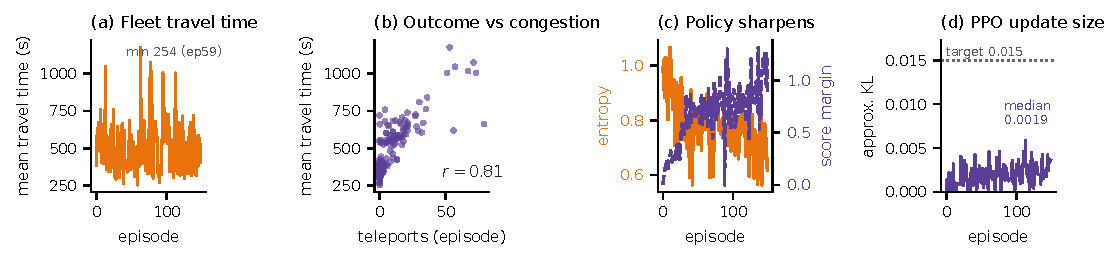
\includegraphics[width=0.98\textwidth]{Images/training_dynamics.pdf}
\caption{MAPPO training over 100 episodes on the congested corridor. (a) Fleet travel time
is highly variable and (b) tracks congestion spikes (teleports): episode outcomes are
demand-driven. (c) Policy entropy anneals as the policy sharpens, but (d) PPO updates stay
well below the target KL, indicating a weak per-update learning signal---the expected
behavior on a low-price-of-anarchy grid.}
\label{fig:training}
\end{figure*}

\subsection{Checkpoint Selection}
Held-out evaluation on seeds 6000--6010 selected the episode-24 checkpoint. There it
completes all vehicles and reduces mean fleet travel time from 597.3\,s (Dijkstra) to
537.0\,s ($-10.1\%$), winning 8 of 11 scenarios, with lower p90 (1035\,s vs 1071\,s) and
fewer deadline misses (208 vs 220). Notably, the deployed greedy policy takes \emph{zero}
non-shortest routes on these seeds---its advantage over Dijkstra comes entirely from
recomputing the shortest route against live congestion, not from visible detours. This
foreshadows the central finding: on this network the fleet benefit and the amount of overt
sacrifice are largely decoupled.

\subsection{Deployment: MAPPO vs.\ Dijkstra}
We deploy the selected checkpoint on 20 held-out scenarios (seeds 4010--4029) against
Dijkstra on identical demand (Table~\ref{tab:deploy}, Fig.~\ref{fig:deploy}). Both complete
100\% of vehicles. Greedy MAPPO---with the detour guard active, our default deployment---%
reduces mean fleet travel time from 596.6\,s to 559.2\,s ($-6.3\%$, median per-scenario
$-22.3$\,s), winning 16 of 20 scenarios, and improves p90 travel time (1062\,s vs 1098\,s)
and deadline misses (214 vs 226). The improvement grows with congestion (correlation
between per-scenario gain and Dijkstra travel time $r{=}-0.48$, Fig.~\ref{fig:deploy}b):
the largest wins are the most congested scenarios---seed~4028 ($1109\to713$\,s) and
seed~4010 ($1585\to1249$\,s)---while the few losses are light-traffic scenarios where the
shortest path is already near-optimal (seeds 4014, 4013 at $+8$\,s each). One scenario,
seed~4012, is a genuine failure: MAPPO nearly doubles travel time ($664\to1191$\,s), a rare
gridlock we return to in Section~V-F.

\begin{table}[!t]
\caption{Deployment over 20 Held-Out Scenarios (Seeds 4010--4029)}
\label{tab:deploy}
\centering
\footnotesize
\setlength{\tabcolsep}{3.4pt}
\begin{tabular}{lrrr}
\toprule
Metric & Dijkstra & \shortstack[r]{MAPPO\\(guard on)} & \shortstack[r]{MAPPO\\(guard off)} \\
\midrule
Completion rate       & 1.000 & 1.000 & 1.000 \\
Avg.\ travel time (s) & 596.6 & 559.2 & \textbf{529.8} \\
\quad vs.\ Dijkstra   & --    & $-6.3\%$ & $\mathbf{-11.2\%}$ \\
p50 travel time (s)   & 576.7 & 541.9 & \textbf{525.9} \\
p90 travel time (s)   & 1097.6 & 1061.8 & \textbf{965.5} \\
Tail gap (steps)      & 596.7 & 587.7 & \textbf{540.9} \\
p95/p50 ratio         & 2.17  & 2.24  & \textbf{2.05} \\
Deadline misses       & 225.8 & \textbf{213.6} & 216.8 \\
Non-shortest rate     & --    & 0.00  & 0.48 \\
Scenarios won         & --    & \textbf{16/20} & 12/20 \\
\bottomrule
\end{tabular}
\end{table}

\begin{figure*}[!t]
\centering
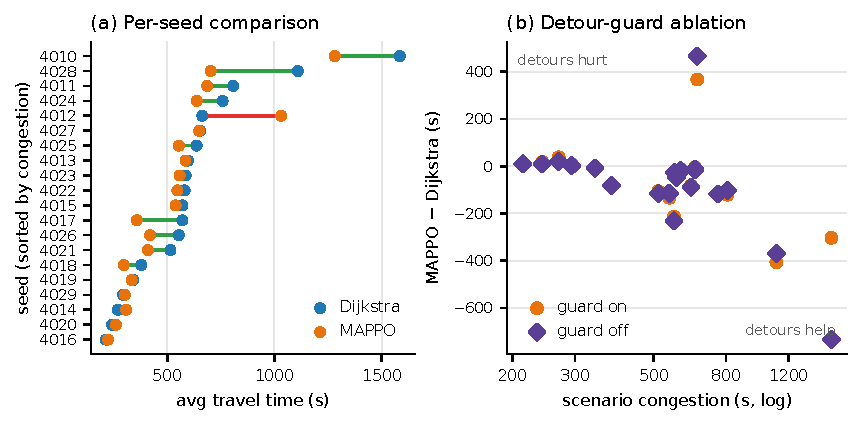
\includegraphics[width=0.98\textwidth]{Images/deployment.pdf}
\caption{Deployment on 20 held-out scenarios. (a)~Per-scenario fleet travel time, Dijkstra
vs.\ greedy MAPPO, sorted by congestion; green connectors mark MAPPO wins, red losses.
(b)~The per-scenario gain grows with congestion ($r{=}-0.48$): MAPPO's largest improvements
are on the most congested scenarios, with the few losses at light traffic and one gridlock
outlier (seed~4012). (c)~Removing the detour guard lets the policy execute its 48\% detours
(violet): these hurt in light traffic (points above zero, left) but help increasingly as
congestion rises (points below the guarded orange, right).}
\label{fig:deploy}
\end{figure*}

\subsection{When Do Selfless Detours Help? A Detour-Guard Ablation}
The default deployment executes zero overt detours, yet the underlying policy is far from
passive. The \emph{detour guard} is a deployment-time filter that keeps a vehicle on the
shortest route when its chosen alternative is already near capacity and the network is
congested. Removing it reveals that the learned policy in fact chooses a non-shortest route
48\% of the time (Table~\ref{tab:deploy}, right column). Executing those detours lowers
mean fleet travel time \emph{further}, to 529.8\,s ($-11.2\%$ vs.\ Dijkstra), and improves
p90 (965.5\,s) and the p95/p50 spread (2.05), because spreading load across alternatives
thins the tail. However, the gain is concentrated entirely at high congestion
(Fig.~\ref{fig:deploy}c): the detours rescue the congested scenarios (seed~4012
$1191\to838$\,s, seed~4010 $1249\to1030$\,s) while \emph{hurting} light-traffic scenarios,
where a longer route only adds distance with no jam to relieve (seeds 4016, 4020, 4014 each
about $+75$\,s). The net effect is that the unguarded policy wins fewer scenarios (12/20)
despite a better mean and tail.

This is the paper's central result. The value of selfless routing is not a fixed property
of the policy; it tracks the network's price of anarchy. Where contention is high, the
learned detours move vehicles off congested corridors onto genuine spare capacity and cut
fleet travel time substantially; where the grid is lightly loaded, selfish shortest-path
routing already approximates the system optimum and every detour is wasted distance. The
detour guard encodes exactly this distinction as a deployment-time robustness knob:
suppressing detours in heavy congestion converts the higher-mean-gain policy into a safer
one that wins more scenarios but forgoes the largest fleet improvements.

\subsection{Greedy vs.\ Stochastic Deployment}
With the detour guard active, greedy (argmax) and stochastic (sampled) deployment produce
identical results on all 20 scenarios. Two effects combine: the trained policy's candidate
scores are sharply peaked (mean margin 1.08), so sampling rarely diverges from the argmax,
and any detour sampling does select is reverted by the guard in this congested regime.
Route diversity---the usual argument for stochastic deployment as a load-spreading
mechanism---is therefore delivered here by the route reservation field and the policy
itself rather than by sampling noise. When the guard is removed the two modes diverge, but
so does the rare gridlock behavior that independent sampling can cause when many vehicles
commit to the same corridor at once.

\subsection{Limitations}
Three limitations qualify these results. First, the aggregate gains are driven by a
minority of severe-congestion scenarios; this is arguably the point of selfless routing,
but it inflates means and widens variance. Second, one scenario (seed~4012) is a true
failure in which the greedy policy gridlocks and the guard does not prevent it, indicating
that the coordination guardrails are necessary but not sufficient. Third, the weak
per-update learning signal (Section~V-A) means the policy is likely under-trained relative
to its ceiling; the low price of anarchy of a dense grid limits how much any routing policy
can gain, which both explains the modest headline number and motivates evaluation on
higher-price-of-anarchy networks. We report these openly because the honest contribution is
the \emph{conditions} under which selfless routing helps, not a single benchmark number.
